\section{A case for application-level inter-DC multicast overlays}
\label{sec:motivation}

We start by providing a case for an application-level multicast
overlay network. We first characterize the inter-DC multicast
workload in \company, a global-scale online service provider
(\Section\ref{subsec:motivation:multicast-traffic}). We then show
the opportunities of improving multicast performance by leveraging
disjoint application-level overlay paths available in geo-distributed
DCs (\Section\ref{subsec:motivation:case-for}). Finally, we examine
\company's current solution of inter-DC multicast (\alg), and draw
lessons from real-world incidents to inform the design of \name
(\Section\ref{subsec:motivation:baseline}). The findings are based on
a dataset of \company's inter-DC traffic collected in a duration of
seven days. The dataset comprises of about 1265 multicast transfers
among 30+ geo-distributed DCs.


\subsection{\company's inter-DC multicast workload}
\label{subsec:motivation:multicast-traffic}


\begin{table}[t!]
\begin{center}
\resizebox{3in}{!}{
%\begin{tabular}{p{2cm}<{\centering}|p{2cm}<{\centering}}
\begin{tabular}{| c | c|}
\hline
 \rowcolor[gray]{0.9}
\textbf{Type of application} & \textbf{\% of multicast traffic} \\
\hline\hline
All applications & 91.13\%~\myfootnotemark\\
\hline
Blog articles & 91.0\% \\% 4648.92 vs 41372.56 in GB
\hline
Search indexing & 89.2\%\\% 16766.7 vs 138418.12
%\hline
%International & 98.15\%\\% 1297.7 vs 68699.97
\hline
Offline file sharing & 98.18\%\\% 2792.4 vs 150234.25
%\hline
%Scholar & 98.09\%\\% 451.22 vs 23134.21
\hline
Forum posts & 98.08\%\\% 964.62 vs 49327.01
\hline
Other DB sync-ups & 99.1\%\\% ?? vs ??
\hline
\end{tabular}
}
\end{center}
\caption{Inter-DC multicast (replicating data from
one DC to many DCs) dominantes \company's inter-DC
traffic.}
%\vspace{-0.2cm}
\label{table:rate}
\end{table}
\myfootnotetext{The overall multicast traffic share is estimated using the traffic that goes through one randomly sampled DC, because we do not have access to information of all inter-DC traffic, but this number is consistent with what we observe from other DCs.}

\mypara{Share of inter-DC multicast traffic}
Table~\ref{table:rate} shows inter-DC multicast (replicating data
from one DC to multiple DCs) as a fraction of all inter-DC traffic.
We see that inter-DC multicast dominates \company's overall inter-DC
traffic (91.13\%), as well as the traffic of individual application
types (89.2 to 99.1\%). The fact that inter-DC multicast traffic
amounts to a dominating share of inter-DC traffic highlights {\em the
importance of optimizing the performance of inter-DC multicast.}

\begin{figure}[t]
        \centering
        \begin{subfigure}[b]{0.23\textwidth}
                \centering
                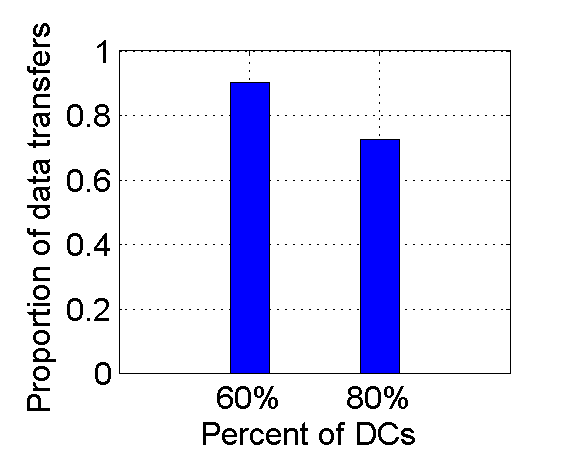
\includegraphics[width=\textwidth]{images/destinationDC_v2.eps}%NeedMulticast.m
                \caption{Proportion of multicast transfers destined to percent of DCs.}
                \label{fig:bulk:dest}
        \end{subfigure}
	\hspace{0.1cm}
        \begin{subfigure}[b]{0.23\textwidth}
                \centering
                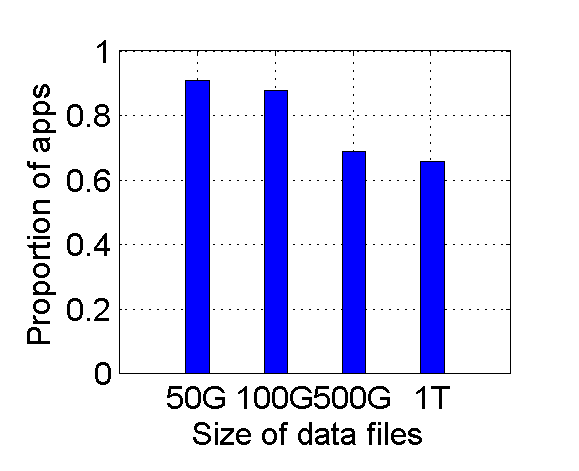
\includegraphics[width=\textwidth]{images/DataSize_v2.eps}
                \caption{Proportion of multicast transfers larger than certain threshold.}
                \label{fig:bulk:size}
        \end{subfigure}
        \vspace{-0.4cm}
        \tightcaption{Inter-DC multicasts (a) are destined to a significant
fraction of DCs, and (b) have large data sizes.}
        \label{fig:bulk}
\vspace{-0.4cm}
\end{figure}

%\vspace{0.1cm}
\noindent{\bf Where are inter-DC multicasts destined?}
Next, we want to know if these transfers are destined to a large
fraction (or just a handful) of DCs, and whether they share common
destinations. Figure~\ref{fig:bulk:dest} sketches the distribution
of the percentage of \company's DCs to which multicast transfers
are destined. We see that 90\% of multicast transfers are destined to
at least 60\% of the DCs, and 70\% are destined to over 80\% of the DCs. Moreover,
we found a great diversity in the source DCs and the sets of destination
DCs (not shown here). These observations suggest that it is untenable
to pre-configure all possible multicast requests; instead, {\em we
need a system to automatically route and schedule any given inter-DC
multicast transfers.}

\mypara{Sizes of inter-DC multicast transfers}
Finally, Figure~\ref{fig:bulk:size} outlines the distribution of data
size of inter-DC multicast. We see that for over 60\% multicast
transfers, the file sizes are over 1TB (and 90\% are over 50GB).
Given that the total WAN bandwidth assigned to each multicast is on
the order of several Gb/s, these transfers are not transient but
persistent, typically lasting for at least tens of seconds.
Therefore, {\em any scheme that optimizes multicast traffic must
dynamically adapt to any performance variation during a data transfer.}
On the flip side, such temporal persistence also implies that {\em
multicast traffic can tolerate a small amount of delay caused by
a centralized control mechanism, such as \name}
(\Section\ref{sec:overview}).


\vspace{0.1cm}
These observations together motivate the need for a systematic approach
to optimizing inter-DC multicast performance.

\subsection{Potentials of inter-DC application-level overlay}
\label{subsec:motivation:case-for}

\begin{figure}[t]
\centering
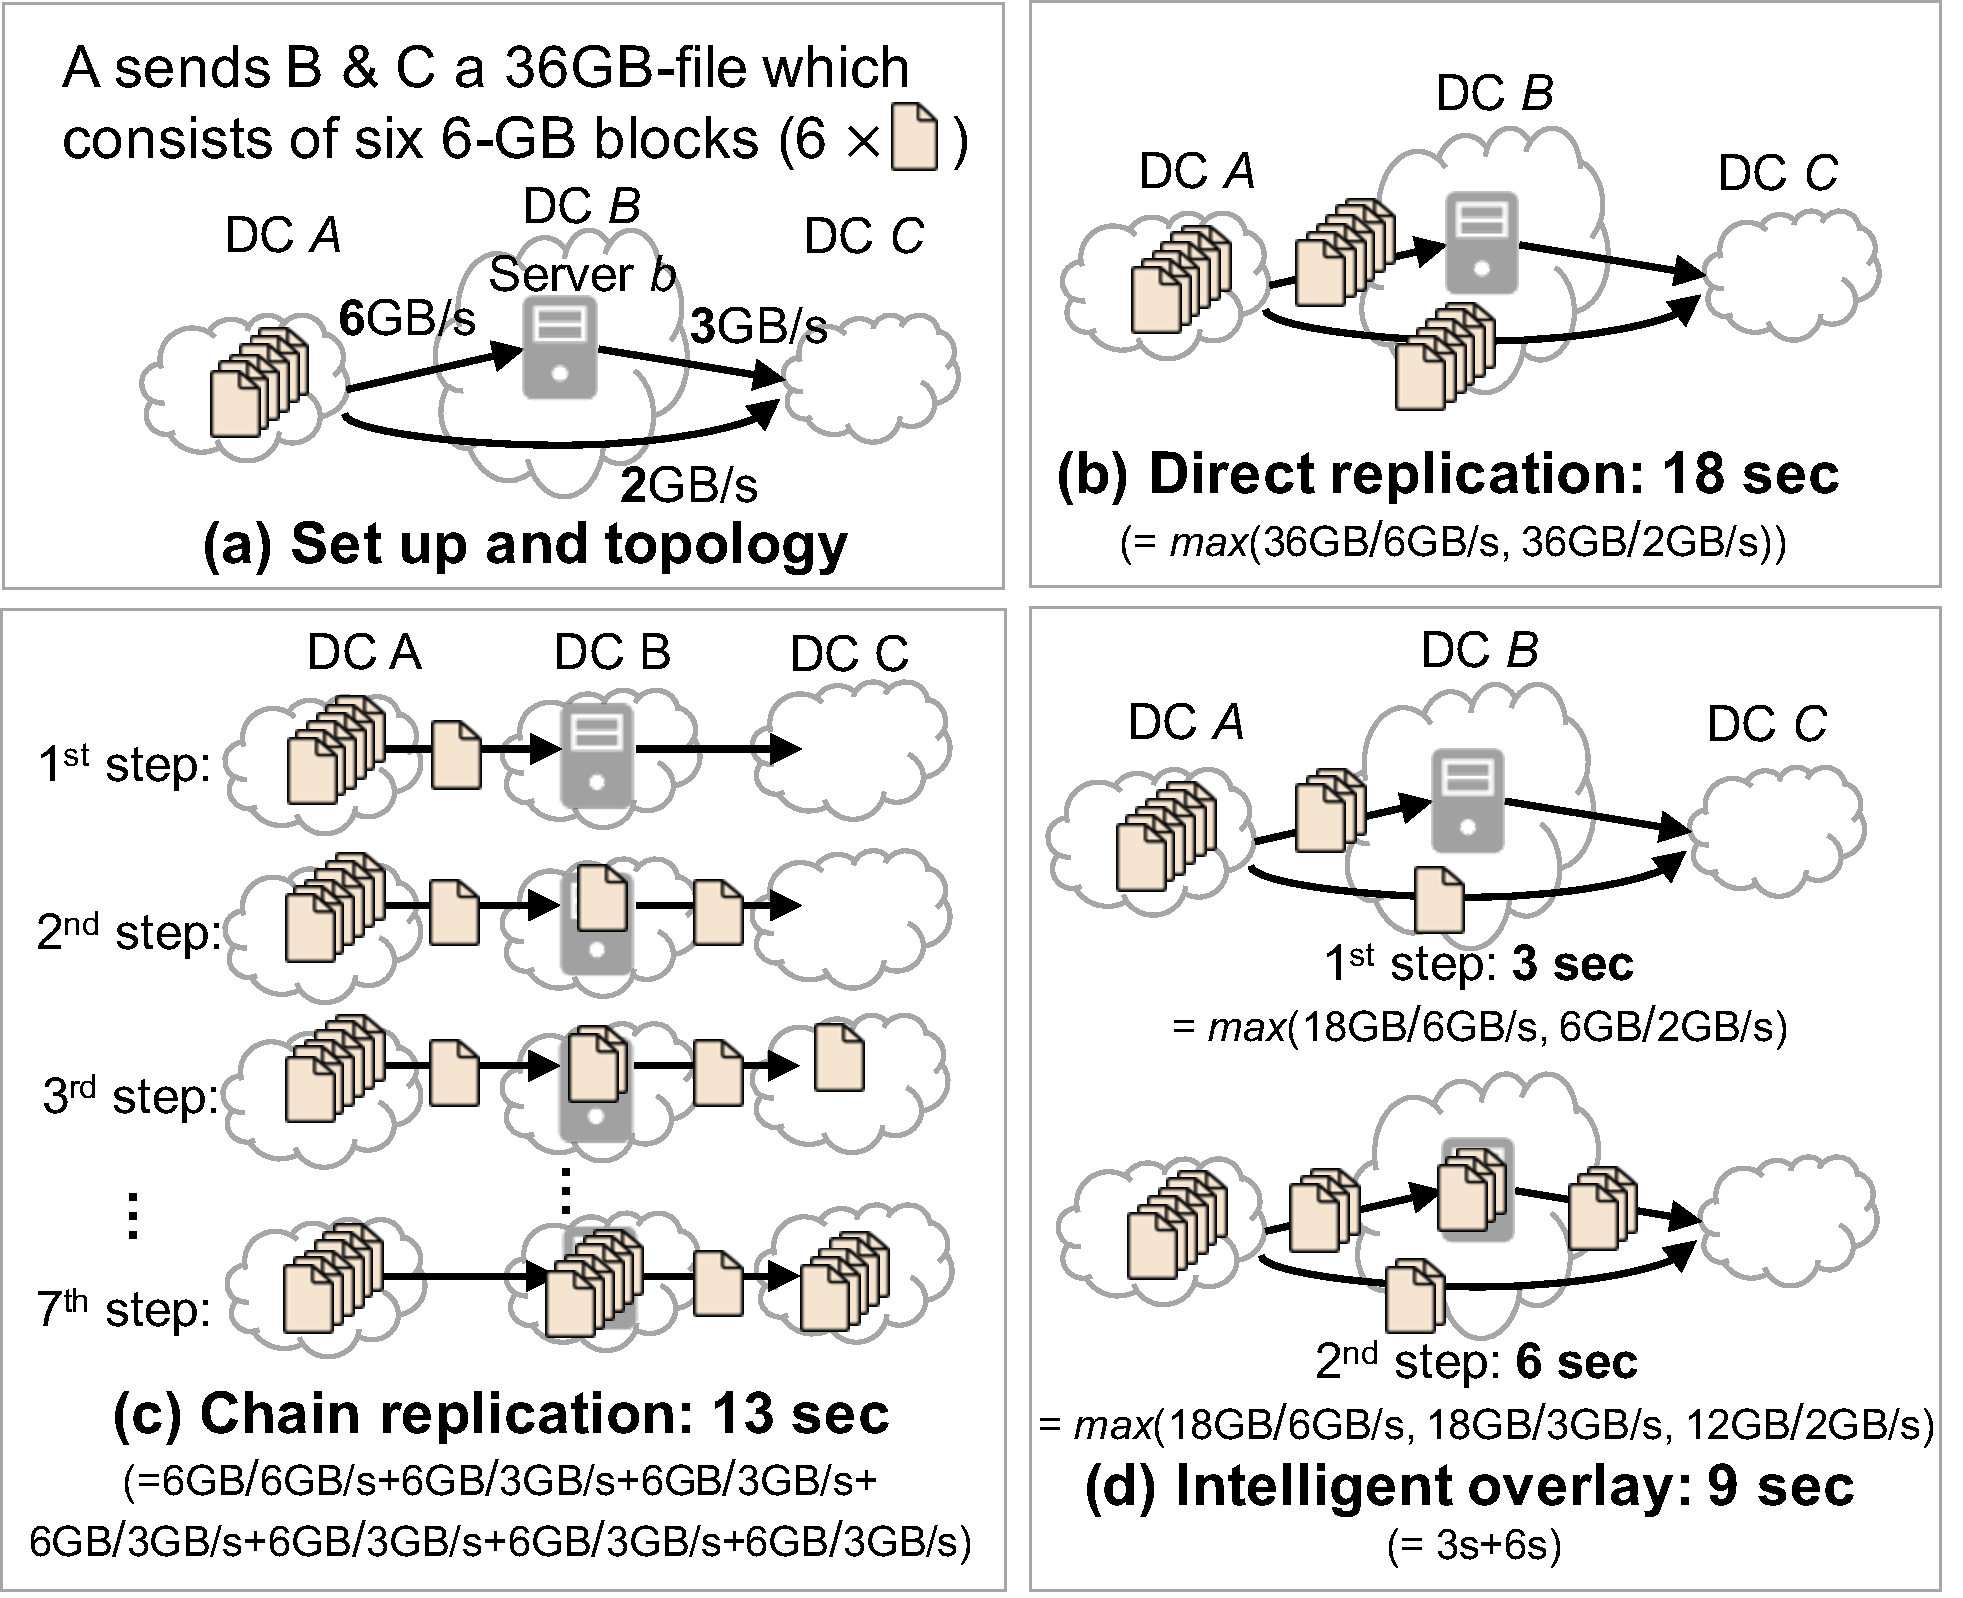
\includegraphics[width=84mm]{images/example-2.pdf}
\vspace{-0.4cm}
\tightcaption{An illustrative example comparing the performance of an intelligent application-level overlay (d) with that of baselines: naive application-level overlay (c) and no overlay (b).}
\label{fig:case:example}
\vspace{-0.4cm}
\end{figure}

It is known that, generally, multicast can be delivered using application-level
overlays~\cite{chu2000case}. Here, we show that inter-DC multicast
completion time (defined by the time until each destination DC has
a full copy of the data) can be greatly reduced by an
application-level overlay network. Note that an application-level
overlay does not require any network-level support, so it is
complementary to prior work on WAN optimization.

The basic idea of an application-level overlay network is to
distribute traffic along {\em bottleneck-disjoint} overlay
paths~\cite{datta19951}, i.e., the two paths do not share a common
bottleneck link or intermediate server.
In the context of inter-DC transfers, two overlay paths either
traverse different sequences of DCs ({\em Type I}), or
traverse different sequences of servers of the same sequence of
DCs ({\em Type II}), or some combination of the two.
%In Type I, the bottleneck can be in intermediate links or inside a DC,
%and in {\em Type II}, the bottleneck is likely to be inside a DC.
Next, we use examples to show bottleneck-disjoint overlay paths can
arise in both types of overlay paths and how they improve inter-DC
multicast performance.

\mypara{Examples of bottleneck-disjoint overlay paths}
In Figure~\ref{fig:intro}, we have already seen how two Type I overlay
paths ($A$$\rightarrow$$B$$\rightarrow$$C$ and
$A$$\rightarrow$$C$$\rightarrow$$B$) are bottleneck-disjoint,
and how it improves the performance of inter-DC multicast.
Figure~\ref{fig:case:example} shows an example
of Type II bottleneck-disjoint overlay paths
(traversing the same sequence of DCs but different sequence of
servers). Suppose we need to replicate 36GB data from DC $A$
to $B$ and $C$ via two bottleneck-disjoint paths:
(1) $A$$\rightarrow$$C$:
from $A$ through $B$ to $C$ using IP-layer WAN routing with
2GB/s capacity, or
(2) $A$$\rightarrow$$b$$\rightarrow$$C$: from $A$ to a server
$b$ in $B$ with
6GB/s capacity and $b$ to $C$ with 3GB/s capacity.
The data is split into six 6GB-blocks.
We consider three strategies.
(1) {\em Direct replication}:
if $A$ sends data directly to $B$ and $C$ via WAN paths
(Figure~\ref{fig:case:example}(b)),
the completion time is 18 seconds.
(2) {\em Simple chain replication}:
a naive use of application-level overlay paths
is to send blocks through server $b$ acting as a
store-and-relay point
(Figure~\ref{fig:case:example}(c)),
and the completion time is 13 seconds (27\% less than without overlay).
(3) {\em Intelligent multicast overlay}:
Figure~\ref{fig:case:example}(d) further improves the performance by
selectively sending blocks along the two paths simultaneously,
which completes in 9 seconds (30\% less than chain replication,
and 50\% less than direct replication).



\begin{figure}[t]
\centering
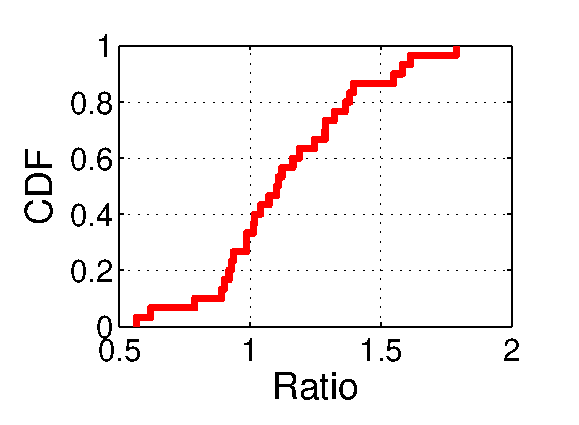
\includegraphics[width=1.5in]{images/potential_v2.eps}%DrawUp.m
\tightcaption{There is a significant performance variance among
the inter-DC overlay paths in our network, indicating that most
pairs of overlay paths are bottleneck disjoint.
%The figure shows the ratio between the available bandwidth
%from $A$ to $C$ through WAN ($BW_{A\rightarrow C}$) and
%that from $A$ to $C$ through $b$
%($BW_{A\rightarrow b\rightarrow C}$),
%across all possible $b$.
}
%\jc{drop (a). avoid using notions in figure captions. captions should be standalone}\jc{please use notations in consistent with those in the text}
\label{fig:case:size}
\vspace{-0.4cm}
\end{figure}

\mypara{Bottleneck-disjoint overlay paths in the wild}
It is hard to identify all bottleneck-disjoint overlay paths in our
network performance dataset, since it does not have per-hop bandwidth information of each
multicast transfer.
Instead, we observe that if two overlay paths have different end-to-end
throughput at the same time, they should be bottleneck-disjoint.
We show one example of bottleneck-disjoint overlay paths in the wild,
which consists of two overlay paths $A$$\rightarrow$$b$$\rightarrow$$C$
and $A$$\rightarrow$$C$, where the WAN routing from DC $A$ to DC $C$ goes
through DC $B$, and $b$ is a server in $B$ (these two paths are
topologically identical to Figure~\ref{fig:case:example}).
If $\frac{BW_{A\rightarrow C}}{BW_{A\rightarrow b\rightarrow C}}\neq1$,
they are bottleneck-disjoint ($BW_p$ denotes the throughput of path $p$).
Figure~\ref{fig:case:size} shows the distribution of
$\frac{BW_{A\rightarrow C}}{BW_{A\rightarrow b\rightarrow C}}$
among all possible values of $A$, $b$, and $C$ in the dataset.
We can see that more than 95\% pairs of $A$$\rightarrow$$b$$\rightarrow$$C$
and $A$$\rightarrow$$C$ have different end-to-end throughput, i.e.,
they are bottleneck disjoint.


\subsection{Limitations of existing solutions}
\label{subsec:motivation:baseline}

Realizing and demonstrating the potential improvement of an application-level
overlay network has some complications. As a first order approximation, we can
simply borrow existing techniques from multicast overlay networks
in other contexts. But the operational experience of \company shows
two limitations of this approach that will be described below.

\mypara{Existing solutions of \company}
To meet the need of rapid growth of inter-DC data replication,
\company has deployed \alg, an application-level overlay network a few
years ago. Despite years of refinement, \alg is based on a
receiver-driven decentralized overlay multicast protocol, which
resembles what was used in other overlay networks (such as CDNs and
overlay-based live video
streaming~\cite{Andreev2013Designing,sripanidkulchai2004analysis,zhang2005coolstreaming}).
The basic idea is that when multiple DCs request a data file from
a source DC, the requested data would flow back through multiple
stages of intermediate servers,  where the selection of senders in
each stage is driven by the receivers of the next stage in a
decentralized fashion.

\noindent{\bf Limitation 1:
Inefficient local adaptation.}
The existing decentralized protocol lacks the global view and thus
suffers from suboptimal scheduling and routing decisions.
To show this, we sent a 30GB file from one DC to two destination
DCs in \company's network. Each DC had 640 servers, each with 20Mbps
upload and download bandwidth (in the same magnitude of bandwidth
assigned to each bulk-data transfer in production traffic).
%\myfootnote{In \company, multiple services are mixed-deployed
%in the same DCs and even in the same servers, so server bandwidth is
%shared by many services and the available bandwidth for bulk data transfer is 20Mbps in general case}.
This 30GB file was evenly stored across all these 640 servers.
Ideally, if the servers select the best source for all blocks, the
completion time will be
$\frac{30\times 1024}{640\times 20Mbps \times 60s/min} = 41$
minutes. But as shown in Figure~\ref{fig:motivation},
servers in the destination DCs on average took 195 minutes (4.75$\times$
the optimal completion time) to receive data, and 5\% of servers even
waited for over 250 minutes.
The key reason for this problem is that individual servers only see a subset of
available data sources (i.e., servers who have already downloaded part of
a file), and thus cannot leverage all available overlay paths to
maximize the throughput. Such suboptimal performance could occur even if
the overlay network is only partially decentralized (e.g.,~\cite{Huang2014A}),
where even if each server does have a global view, local adaptations by
individual servers would still create potential hotspots and congestion on
overlay paths.


\begin{figure}[t]
  \centering
  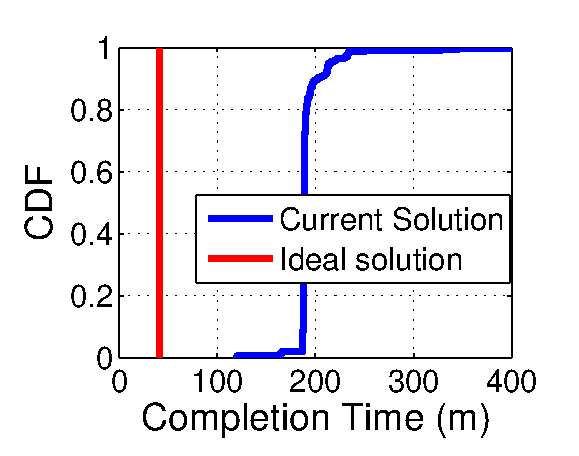
\includegraphics[width=1.5in]{images/SEvsIdeal.eps}
  \vspace{-0.2cm}
  \tightcaption{The CDF of the actual flow completion time at different servers in the destination DCs,
compared with that of the ideal solution. }
  \label{fig:motivation}
\vspace{-0.4cm}
\end{figure}


\NEW{
\noindent{\bf Limitation 2: High computation overhead.} To obtain a global view and achieve optimal scheduling protocols, the existing centralized protocols suffers from high computation overhead. Most formulations are super-linear, so the computational overhead of centralized protocols always grows exponentially, making them intractable in practice.

\noindent{\bf Limitation 3: Interaction with latency-sensitive traffic.}
The existing multicast overlay network shares the same inter-DC WAN
with latency-sensitive traffic. Despite using standard QoS techniques,
and giving the lowest priority to bulk data transfers, we still see
negative impacts on latency-sensitive traffic by bursty arrivals of
bulk-data multicast requests. Figure~\ref{fig:lesson2} shows the
bandwidth utilization of an inter-DC link in two days during which a
6-hour long bulk data transfer started at 11:00pm on the second day.
The blue line denotes the outgoing bandwidth, and the green line
denotes the incoming bandwidth. We can see that the
bulk data transfer caused excessive link utilization (i.e., exceeding
the safety threshold of 80\%), and as a result, the latency-sensitive
online traffic experienced over 30$\times$ delay inflation. Therefore, an algorithm should be able to dynamically interact with latency-sensitive traffic.
}


%The reason is that although all the servers worked under the standard QoS requirements, the excessive bandwidth usage of the inter-DC link still cannot be prevented due to lack of global coordination.


\begin{figure}[t!]
        \center
        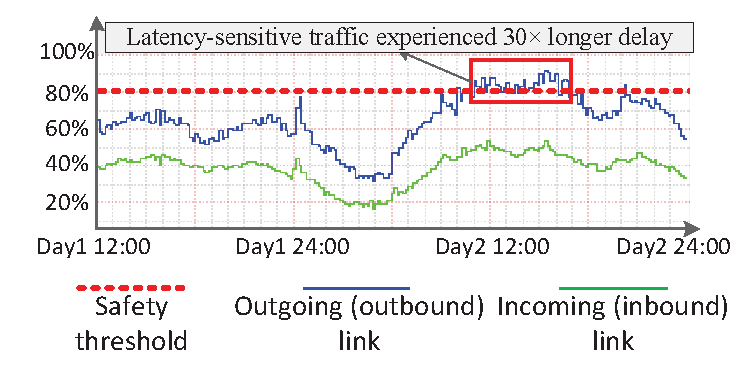
\includegraphics[width=3in]{images/nj02-M2A_0212-0216_v3.eps}
        \tightcaption{The utilization of the inter-DC link in two days. Inter-DC bulk data transfer on the 2nd day caused severe interference on latency-sensitive traffic.}
        \label{fig:lesson2}
\vspace{-0.4cm}
\end{figure}

\subsection{Key observations}
The key observations from this section are following:
\begin{packeditemize}
\item {\em Inter-DC multicasts} amount to a substantial fraction of
inter-DC traffic, have a great variability in source-destination, and
typically last for at least tens of seconds.
\item {\em Bottleneck-disjoint overlay paths} are widely available
between geo-distributed DCs.
\item Existing solutions that rely on local adaptation can have
{\em suboptimal performance} and {\em negative impact on
online traffic}.
\NEW{
\item {\em Real-time dynamic bandwidth separation} can be achieved if: online traffic can be predicted accurately and rescheduling can be conducted accordingly.
}
\end{packeditemize}

%\jc{can you say something like: such inefficiency is due to the inability
%to prevent exceeding bandwidth usage by bulk-data transfers in a
%decentralized manner}
%(1) Use a figure to show that bulk data transfer can cause significant delay on latency-sensitive traffic, and (2) put some concrete numbers to show such delay can cause significant revenue loss.

%\jc{can we show some numbers on how much delay on latency-sensitive traffic during that incident? and how much losses did it cause (either in terms of application quality or in \$\$)?}

%\end{itemize}

